\documentclass[11pt]{article}
\usepackage[margin=1in]{geometry}
\usepackage{graphicx,booktabs,amsmath,microtype,xcolor}
\usepackage[hidelinks]{hyperref}
\usepackage{caption}
\captionsetup{font=small,labelfont=bf}
\graphicspath{{../results_run6/}}
\newcommand{\PC}{\textit{PC}}
\title{Recovering blocking errors with an optimized LLM pipeline:\\results}
\date{}
\begin{document}
\maketitle

\section{Results}

\subsection{Setup recap}

A blocker partitions two record tables into mutually exclusive blocks. At a
realistic operating point it separates many true matches, and those separations
are irrecoverable by any downstream matcher: a pair that never enters the
candidate set can never be labelled. We measure everything on the candidate-set
plane, so the quantity of interest is pair completeness (\PC), the fraction of
gold matching pairs whose two records share a block.

We assume a small number of blocker errors are known---\emph{seed pairs}. A
seed identifies a pair of blocks that provably contains at least one error;
the system is shown the contents of those two blocks together with the seed and
must recover the \emph{other} matching pairs hidden in them. Two components do
this work and both are optimized automatically by GEPA: a \textbf{retrieval
stage} (Python code that reads the full contents of the two blocks and composes
the entire message the judge sees) and a \textbf{judge prompt} (the instruction
that model follows). The judge is Qwen3-8B running locally; the reflection model
that rewrites both components is Claude Sonnet. Optimization used $5{,}010$
task-model rollouts and produced $58$ candidates.

Two controls define the experiment. First, the optimizer is \textbf{blind}: the
reflection model is never told which dataset or which blocking method an episode
came from, every record excerpt it reads has dataset-specific tokens replaced by
placeholders, and a leakage gate rejects proposals containing data-derived
strings. Second, generalization is tested \textbf{across datasets}, not across
held-out episodes of the training datasets: four datasets (amazon--google,
walmart--amazon, dblp--acm, fodors--zagats) form the training bank and two
(abt--buy, dblp--scholar) are touched exactly once, after the run is frozen.

Table~\ref{tab:bank} gives the base operating point. The blocker is
$\Lambda$-fold LSH with $\Lambda=1$, whose granularity parameter $K$ is tuned
per dataset so that $\PC\approx0.6$: an imperfect blocker, deliberately.

\begin{table}[t]
\centering\small
\begin{tabular}{lrrrrrl}
\toprule
dataset & $K$ & base \PC & gold pairs & separated & episodes & role\\
\midrule
amazon--google  & 8  & 0.597 & 1{,}300 & 524   & 70  & train\\
walmart--amazon & 8  & 0.612 & 1{,}154 & 448   & 73  & train\\
dblp--acm       & 6  & 0.632 & 2{,}224 & 819   & 66  & train\\
fodors--zagats  & 15 & 0.705 & 112     & 33    & 4   & train\\
\midrule
abt--buy        & 6  & 0.552 & 1{,}097 & 492   & 58  & \textbf{held out}\\
dblp--scholar   & 6  & 0.592 & 5{,}347 & 2{,}183 & 175 & \textbf{held out}\\
\bottomrule
\end{tabular}
\caption{Base blocking. ``Separated'' counts gold pairs whose records the
blocker placed in different blocks; these are the errors the pipeline is asked
to repair.}
\label{tab:bank}
\end{table}

\subsection{What the optimizer produced}

Figure~\ref{fig:opt} shows the run. The seed candidate---a naive retrieval stage
that emits every record of both blocks in identifier order, and a six-line task
statement---scores $0.033$ on the mixed validation bank. Optimization ends at
$0.355$, a tenfold improvement, and eleven candidates set a new best along the
way.

The shape of that curve is the first result. The three largest relative gains
($+160\%$, $+125\%$, $+30\%$, all within the first $400$ rollouts) come from
rewrites of the \emph{retrieval code}, not the prompt; prompt rewrites
contribute the middle band ($+5\%$, $+3\%$, $+9\%$). The asymmetry is
mechanical: a judging instruction cannot recover a pair whose records never
reached the message, so the coverage ceiling has to be lifted before wording
matters. Systems that optimize the prompt alone are bounded by whatever
retrieval they were handed.

\begin{figure}[t]
\centering
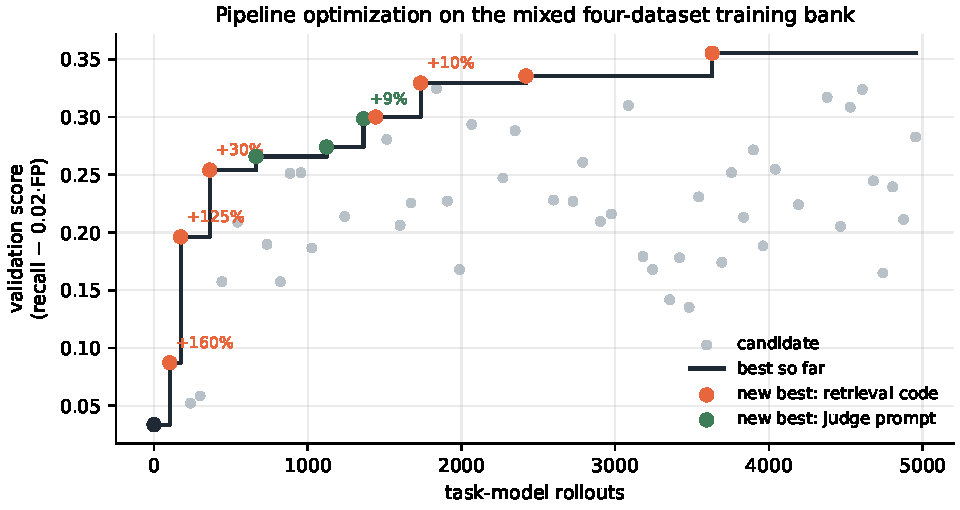
\includegraphics[width=\linewidth]{fig1_optimization.pdf}
\caption{Validation score against task-model rollouts. Points are candidates;
the step line is the running best. Coloured markers are new bests, coloured by
which component the reflection model rewrote. The early, large gains are all
retrieval-code rewrites.}
\label{fig:opt}
\end{figure}

\subsection{Held-out datasets}

Table~\ref{tab:heldout} and Figure~\ref{fig:pc} give the frozen, single-pass
result on the two datasets that never appeared in training. The naive seed
pipeline recovers $42$ of $2{,}277$ hidden pairs ($1.8\%$); the optimized
pipeline recovers $1{,}037$ ($45.5\%$), a $24.7\times$ improvement, at a cost of
$3{,}276$ false candidate pairs---roughly three added pairs per repaired one,
far inside the customary budget of one percent of the candidate set.

\begin{table}[t]
\centering\small
\begin{tabular}{lrrrr}
\toprule
pipeline & recovered & recall & coverage & false positives\\
\midrule
naive seed (\#0)        & 42/2{,}277    & 1.8\%  & 197   & 1{,}118\\
midpoint (\#16)         & 553/2{,}277   & 24.3\% & 989   & 3{,}485\\
\textbf{optimized (\#41)} & \textbf{1{,}037/2{,}277} & \textbf{45.5\%} & 1{,}609 & 3{,}276\\
\bottomrule
\end{tabular}
\caption{Held-out bank (abt--buy $+$ dblp--scholar; $233$ episodes,
$2{,}277$ hidden pairs). ``Coverage'' counts hidden pairs whose \emph{both}
records reached the judge's message; a pair outside coverage cannot be found at
any prompt quality.}
\label{tab:heldout}
\end{table}

Expressed on the blocking plane, the repair moves abt--buy from
$\PC=0.552$ to $0.691$ ($+13.9$ points) and dblp--scholar from $0.592$ to
$0.758$ ($+16.6$ points), using an 8B model on one consumer GPU.

\begin{figure}[t]
\centering
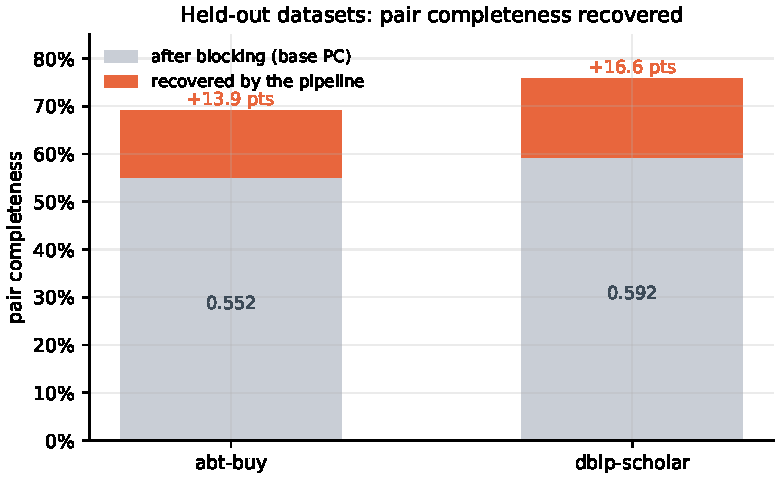
\includegraphics[width=0.62\linewidth]{fig2_heldout_pc.pdf}
\caption{Pair completeness on the two held-out datasets: what the blocker
achieved alone (grey) and what the optimized pipeline restored on top (orange).}
\label{fig:pc}
\end{figure}

\subsection{In-distribution selection predicts out-of-distribution gain}

Because candidates are selected on validation episodes drawn from the
\emph{training} datasets, a natural worry is that the selection signal rewards
dataset-specific behaviour. Figure~\ref{fig:ckpt} tests this by evaluating three
checkpoints---the seed, the midpoint, and the final winner---on the held-out
bank. Validation score, held-out recall and held-out coverage move together
($0.033\to0.298\to0.355$; $1.8\%\to24.3\%\to45.5\%$; $197\to989\to1{,}609$).
There is no point at which validation improves while transfer degrades.

The coverage column is the mechanism made visible: the optimizer's gains come
first from getting the right records in front of the judge, and only then from
judging them better. Between the midpoint and the final candidate, coverage
grows by $63\%$ while recall grows by $87\%$, so the last stretch reflects both
better retrieval and better judgement.

\begin{figure}[t]
\centering
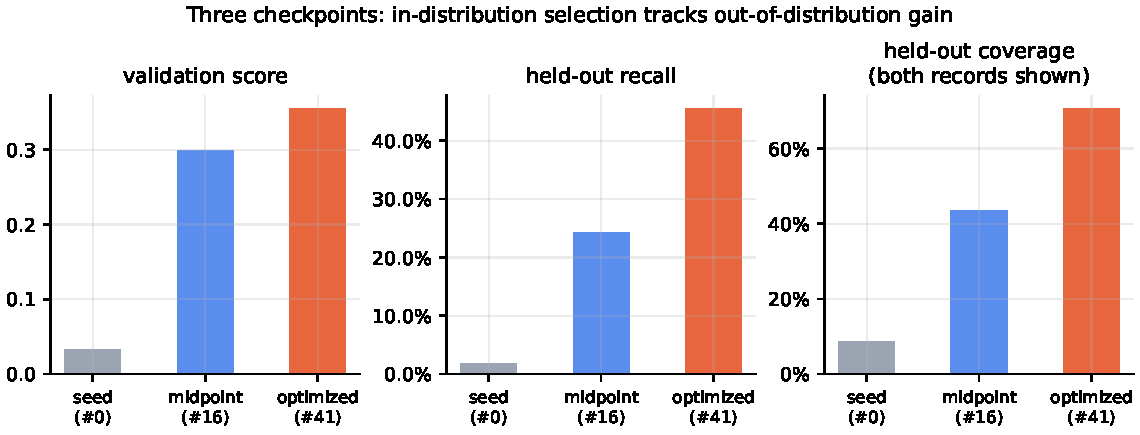
\includegraphics[width=\linewidth]{fig3_checkpoints.pdf}
\caption{Three checkpoints of the same run. Left: score on the mixed validation
bank (training datasets). Middle and right: recall and coverage on the held-out
datasets, which the optimizer never saw.}
\label{fig:ckpt}
\end{figure}

An instructive detail sits inside the aggregate: the midpoint candidate is
\emph{better} on abt--buy ($186/376$) than the final one ($152/376$), but far
worse on dblp--scholar ($367$ versus $885$ of $1{,}901$). The later retrieval
rewrites bought robustness at scale---dblp--scholar episodes reach
$430\times15{,}047$ records---at a small cost on the smaller, cleaner dataset.

\subsection{What the pipeline learned}

The final retrieval stage is a compact meta-blocking engine, written by a model
that was never told what the records were about: it concatenates whatever fields
exist (schema-agnostic), builds an inverted index over rare tokens, scores each
record by the strength of its best potential partner on the other side in both
directions with IDF weighting, models the character cost of its own rendered
output, and allocates the message budget between the two blocks by water-filling.
None of these ideas were supplied; the seed version simply printed everything.

The judge prompt evolved in the complementary direction, from a six-line task
statement into a rubric phrased entirely in structural terms---core identifying
field versus secondary field, variant and edition markers, distinctive versus
boilerplate tokens---and then \emph{shrank} again (3{,}694 to 2{,}462
characters) as the retrieval stage improved and fewer defensive rules were
needed. A content audit finds three data-derived tokens in the final prompt
(\texttt{boilerplate}, \texttt{debugging}, \texttt{descriptor}), all generic
method vocabulary and no dataset entities, against seven (including
\texttt{reseller} and \texttt{sku}) in a comparable run whose reflection model
was allowed to see the data unmasked.

\subsection{What the design cannot reach}

Not every blocker error is addressable by this construction. An episode requires
a block pair containing at least two separated gold pairs: one is revealed as
the seed, the remainder are the targets. Errors that sit alone in their block
pair---\emph{orphans}---yield no episode and are never shown to the system.
Figure~\ref{fig:pop} decomposes each dataset's errors accordingly.

\begin{figure}[t]
\centering
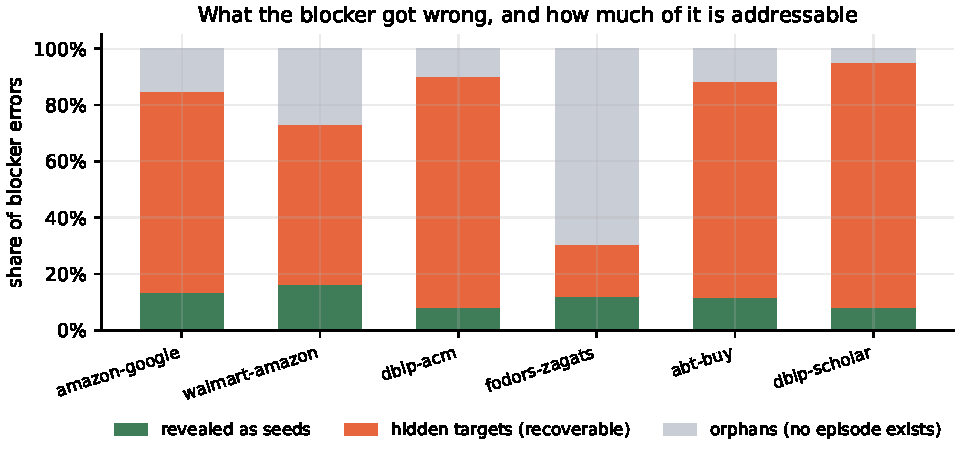
\includegraphics[width=\linewidth]{fig4_error_population.pdf}
\caption{Decomposition of the blocker's errors per dataset: revealed seeds,
hidden targets (the recoverable population), and orphans, which no episode
covers.}
\label{fig:pop}
\end{figure}

Across the bank, $9.9\%$ of errors are revealed as seeds, $79.7\%$ are
recoverable targets, and $10.4\%$ are orphans. On the held-out datasets the
orphan share is $11.8\%$ (abt--buy) and $4.9\%$ (dblp--scholar). Reporting
recall against the target population, as Table~\ref{tab:heldout} does, therefore
measures the pipeline; measured instead against every error not given away, the
optimized pipeline recovers $1{,}037/2{,}442 = 42.5\%$, and against all
separated pairs including the seeds, $1{,}037/2{,}675 = 38.8\%$.

\subsection{Limitations}

Three bound the claims above. \textbf{One blocker family:} every episode comes
from $\Lambda$-fold LSH, so generality across blocking \emph{methods} is
untested; banks for standard blocking, KLSH and a SimCSE--Louvain blocker are
built and a mixed-blocker run is the immediate next step. \textbf{Seed-driven
triage:} the system is told which block pairs to examine, so the results
describe repair given correct triage, not discovery of blocking errors from
scratch. \textbf{Selection noise:} the winner is the best of $58$ candidates
chosen on $55$ validation episodes; the margin over the naive baseline is far
outside noise, but small differences between late candidates are not
confirmatory. Separately, we note a data defect found and fixed during this
work: walmart--amazon reuses one identifier space across both of its tables,
which silently merged records in an earlier bank build; that dataset is in the
training split only, and the held-out results reported here are unaffected.

\subsection{Reproducibility}

Every rollout and every reflection call---prompts and raw responses---is logged;
all $58$ candidates are stored with their lineage; retrieval stages are
deterministic per episode, so the message any checkpoint produced can be
regenerated exactly rather than reconstructed.

\end{document}
